% -*- coding:utf-8 -*-

\chapter{第一章}
\zhlipsum* 正文正文正文\cite{zhang_study_2013}。

\section{二级标题}
正文正文正文正文\cite{chen_problem-solving_2019,dasgupta_handbook_2018}。
\zhlipsum*
正文正文正文正文\cite{barberis_survey_2003,heckman_chapter_2007,__2014}。
正文正文正文正文正文\cite{__2015}。

如图\ref{fig:co2}所示,\zhlipsum*[1]
详情参见\cite{yin_quantifying_2019}。

\begin{figure}[H]
  \adjustbox{center}{%
    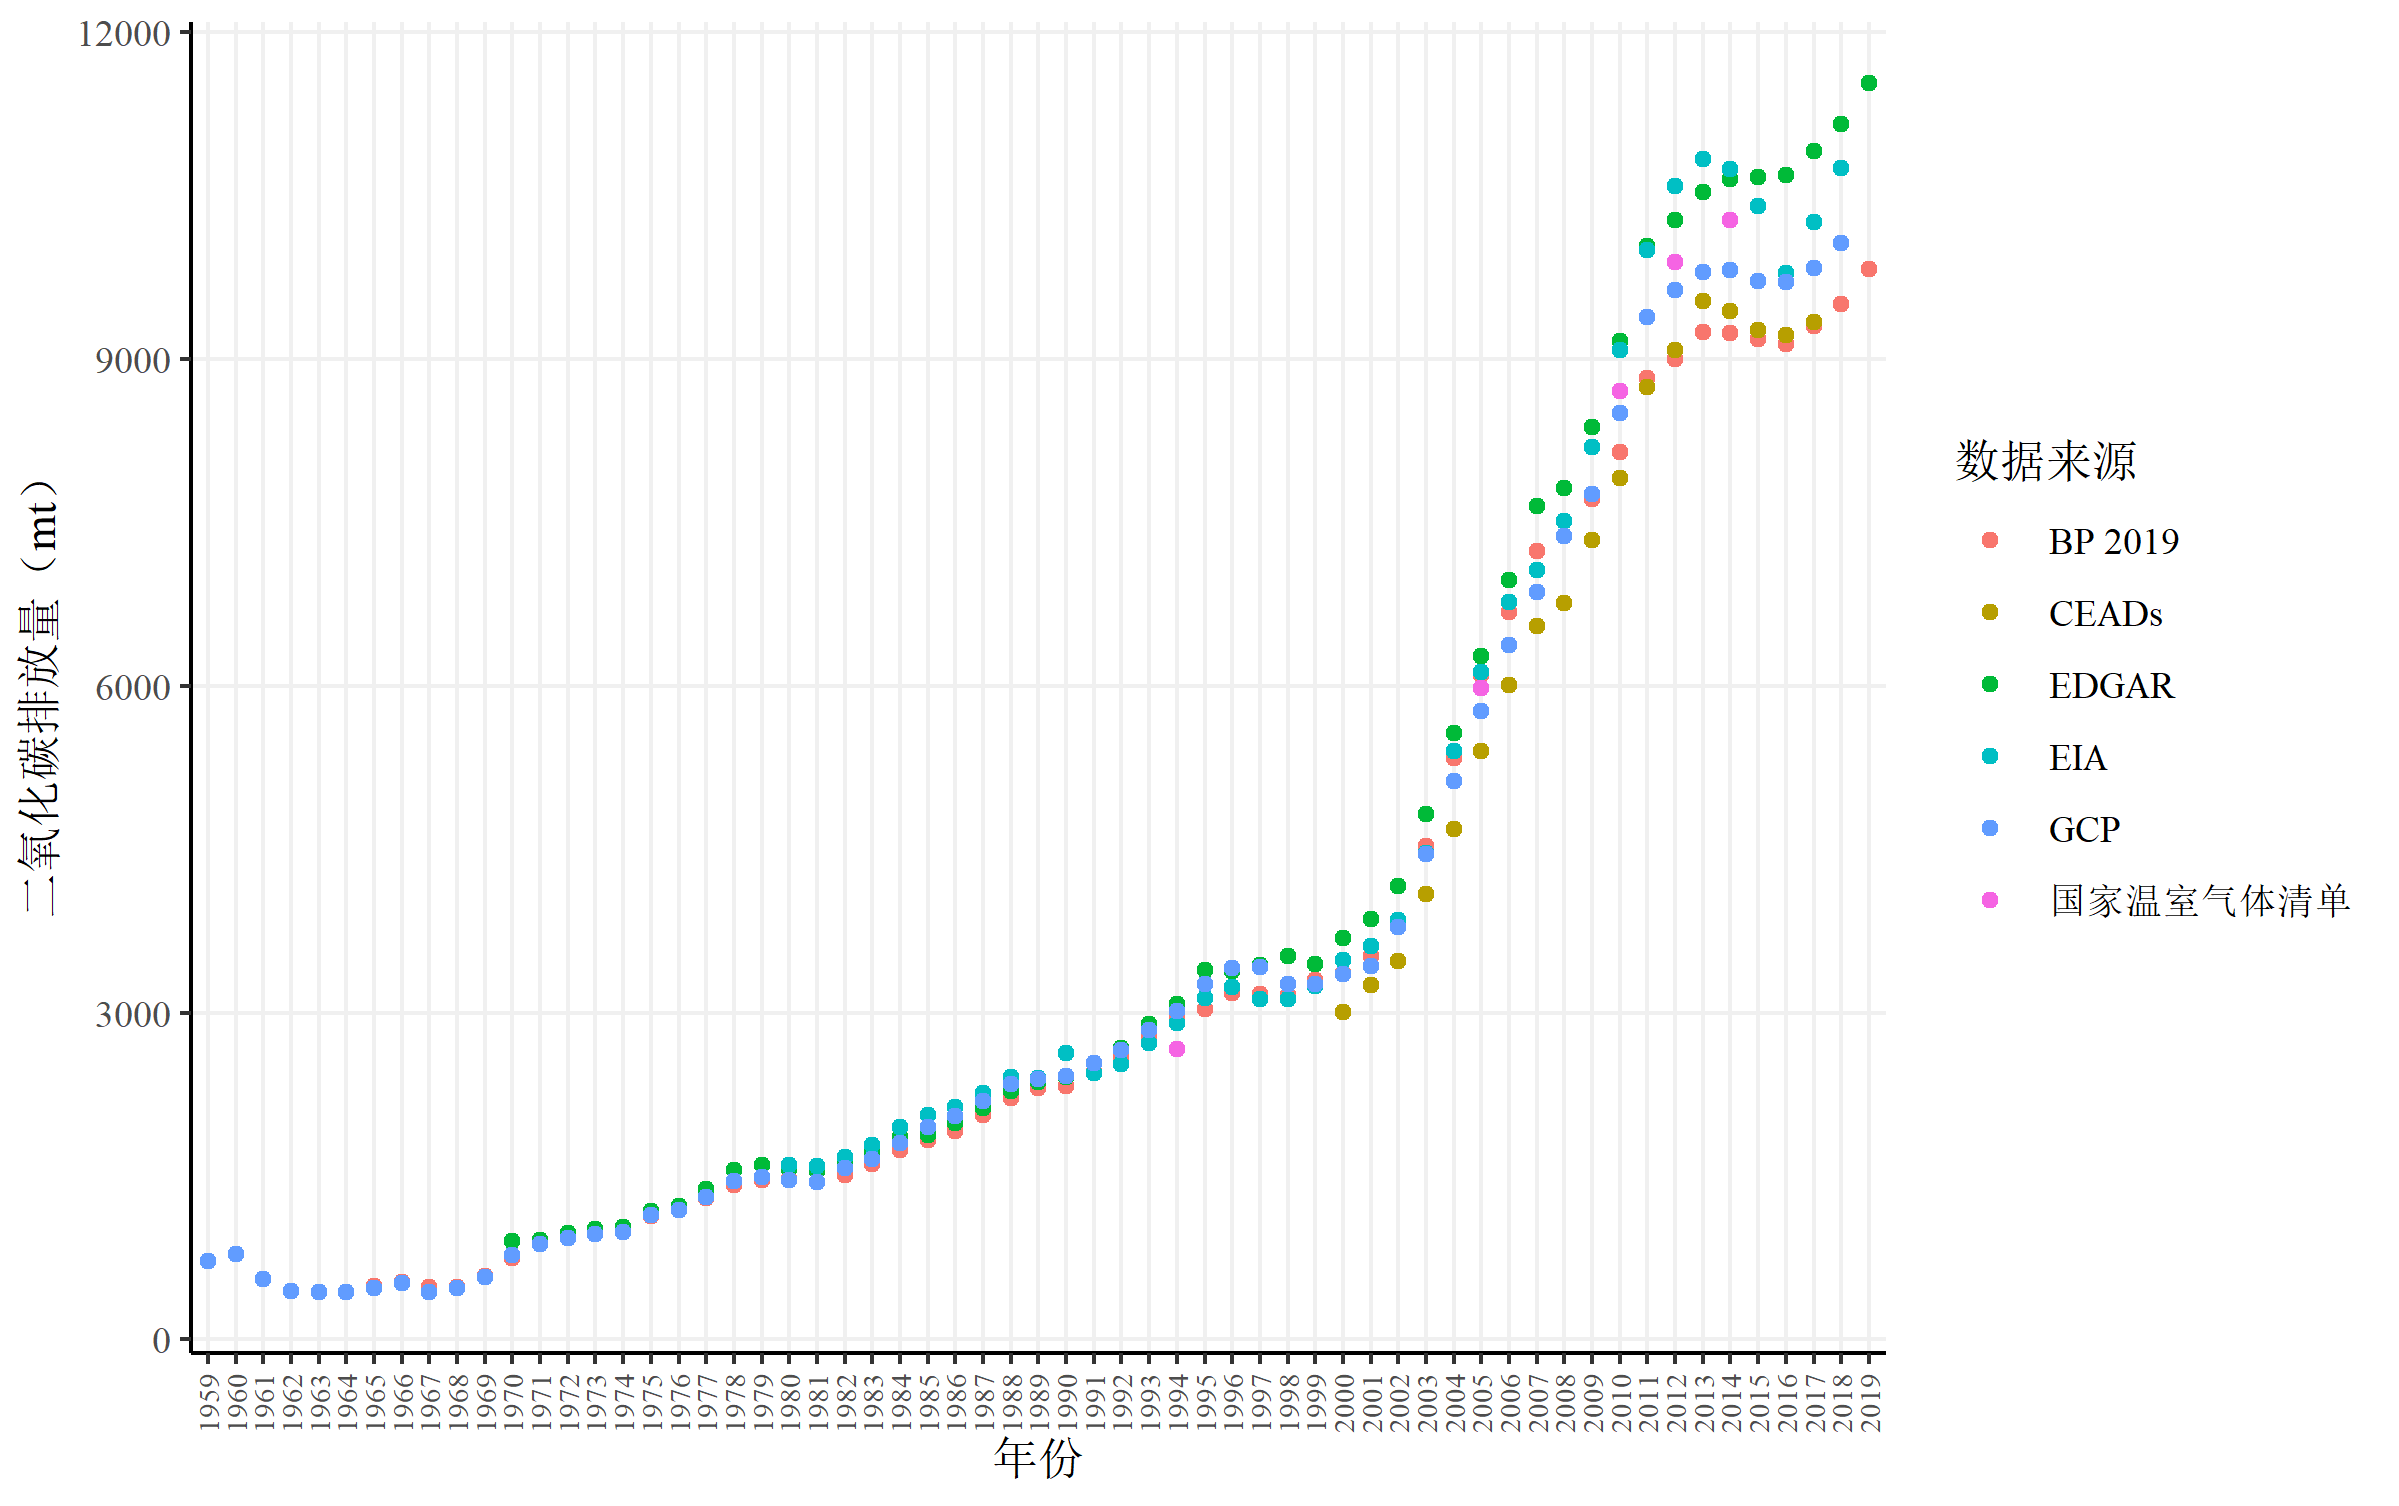
\includegraphics[width=5in]{emission.png}}
  \caption{中国1959-2019年二氧化碳排放量\label{fig:co2}}
  \vspace{1.5ex}
  \begin{minipage}{\textwidth}
    \small
    \phantom{缩进}注:如有需要可对图片进行注释说明,可省略。
    如有需要可对图片进行注释说明,可省略。
    如有需要可对图片进行注释说明,可省略。\\
    \phantom{缩进}图片来源:如需对图片来源进行说明,请参照此格式,可省略。
    如需对图片来源进行说明,请参照此格式,可省略。
  \end{minipage}
\end{figure}
\vspace{-3ex}
\zhlipsum

\subsection{三级标题}
\zhlipsum* 进一步阅读\cite{__2017,schmitt-grohe_covid-19_2020,__2020,__2019}。







